\clearpage
\subsection{premi/client/userManager}
%diagramma del package%
\begin{figure}[h]
\begin{center}
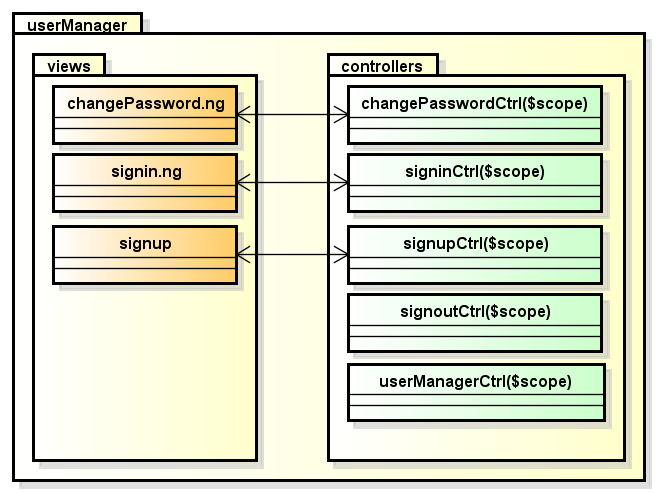
\includegraphics[scale=0.50]{img/diapkg/userManager.png}
\caption{Diagramma del package premi/client/userManager}
\end{center}
\end{figure}



%-------  diagramma di un template %
\subsubsection{premi/client/userManager/views/changePassword.ng}

\begin{description}
%-------  descrizione del template%
\item[Descrizione] \hfill
	Template della vista associata allo \textit{\$scope} di \textit{changePasswordCtrl}. Permette il cambio della password dell'utente
\item[Note] \hfill
	\begin{itemize}
			\item prevede input per l'inserimento dell'email, della vecchia password, della nuova password, e della conferma della nuova password
			\item prevede due pulsanti, uno per confermare il cambio password, l'altro per annullare il cambiamento e tornare alla pagina principale dell'applicazione
	\end{itemize}
\end{description}

%-------  diagramma di un template %
\subsubsection{premi/client/userManager/views/signin.ng}

\begin{description}
%-------  descrizione del template%
\item[Descrizione] \hfill
	Template della vista associata allo \textit{\$scope} di \textit{signinCtrl}. Permette all'utente di effettuare il login e di entrare nell'applicazione
\item[Note] \hfill
	\begin{itemize}
			\item prevede due input, per l'inserimento dell'email e della password
			\item prevede due pulsanti, uno per effettuare il login, l'altro per passare alla pagina di registrazione nel caso in cui l'utente non sia ancora registrato
	\end{itemize}
\end{description}


%-------  diagramma di un template %
\subsubsection{premi/client/userManager/views/signup.ng}

\begin{description}
%-------  descrizione del template%
\item[Descrizione] \hfill
	Template della vista associata allo \textit{\$scope} di \textit{signupCtrl}. Permette all'utente di registrarsi nel database, inserendo email e password
\item[Note] \hfill
	\begin{itemize}
			\item prevede tre input, per l'inserimento dell'email, della password e della conferma della password
			\item prevede due pulsanti, uno per registrarsi, l'altro per effettuare il login nel caso in cui l'utente sia già registrato
			\item se l'utente è già registrato segnala la presenza dell'email all'interno del database
	\end{itemize}
\end{description}


%-------  diagramma di un template %
\subsubsection{premi/client/userManager/views/userManager.ng}

\begin{description}
%-------  descrizione del template%
\item[Descrizione] \hfill
	Genera una vista per indirizzare l'utente alle varie opzioni di gestione dell'account (signin, signout, cambio password)
\end{description}

















%-------  diagramma della classe%
\subsubsection{premi/client/userManager/controllers/changePasswordCtrl}
\begin{figure}[h]
\begin{center}
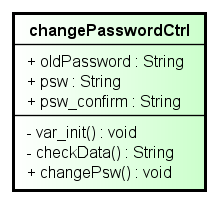
\includegraphics[scale=0.55]{img/diacla/changePasswordCtrl.png}
\caption{Diagramma della classe premi/client/userManager/controllers/changePasswordCtrl}
\end{center}
\end{figure}


\begin{description}
%-------  descrizione della classe%
\item[Descrizione] \hfill
	Controller della view \textit{changePassword.ng}. Permette all'utente di cambiare la password del suo account
	
	
	
%-------  lista delle classi associate%	
\item[Dipendenze] \hfill
	\begin{itemize}
		\item \textbf{premi/client/lib/toastMessageFactory}: per l'invio di notifiche o messaggi di errore all'utente
	\end{itemize}
	
	
%-------  lista degli Attributi%	
\item[Attributi] \hfill
	\begin{description}
		\item[\textbf{+ oldPassword : String			}] \hfill
			La vecchia password dell'account, inserita dall'utente nell'apposito input
		\item[\textbf{+ psw : String			}] \hfill
			La nuova password dell'account, inserita dall'utente nell'apposito input
		\item[\textbf{+ psw\_confirm : String			}] \hfill
			Conferma della nuova password dell'account, inserita dall'utente nell'apposito input
	\end{description}
	
	
%-------  lista dei metodi%	
\item[Metodi] \hfill

	% -- inizio metodo -- %
	\begin{description}
		\item[\textbf{\color{blue}- var\_init() : void			}] \hfill
			Inizializza a stringhe vuote oldPassword, psw e psw\_confirm
	\end{description}
	% -- fine metodo -- %		
	
	% -- inizio metodo -- %
	\begin{description}
		\item[\textbf{\color{blue}- checkData() : String			}] \hfill
			Controlla che le informazioni scritte dall'utente siano corrette. Restituisce una stringa vuota se corrette, o una descrizione sull'errore rilevato se incorrette
	\end{description}
	% -- fine metodo -- %	
	
	% -- inizio metodo -- %
	\begin{description}
		\item[\textbf{\color{blue}+ changePsw() : void			}] \hfill
			Effettua il cambio di password sfruttando il metodo changePassword di \$meteor
			Se sono presenti errori invia un messaggio tramite toastMessageFactory
	\end{description}
	% -- fine metodo -- %	

\end{description}






%-------  diagramma della classe%
\subsubsection{premi/client/userManager/controllers/signinCtrl}
\begin{figure}[h]
\begin{center}
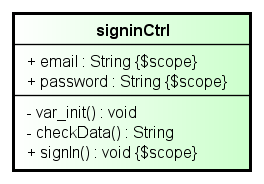
\includegraphics[scale=0.55]{img/diacla/signinCtrl.png}
\caption{Diagramma della classe premi/client/userManager/controllers/signinCtrl}
\end{center}
\end{figure}


\begin{description}
%-------  descrizione della classe%
\item[Descrizione] \hfill
	Controller della view \textit{signin.ng}. Permette all'utente di effettuare il login
	
	
	
%-------  lista delle classi associate%	
\item[Dipendenze] \hfill
	\begin{itemize}
		\item \textbf{premi/client/lib/toastMessageFactory}: per l'invio di notifiche o messaggi di errore all'utente
	\end{itemize}
	
	
%-------  lista degli Attributi%	
\item[Attributi] \hfill
	\begin{description}
		\item[\textbf{+ email : String			}] \hfill
			L'email con cui l'utente si è registrato nel database dell'applicazione
		\item[\textbf{+ password : String			}] \hfill
			La password dell'account dell'utente
	\end{description}
	
	
%-------  lista dei metodi%	
\item[Metodi] \hfill

	% -- inizio metodo -- %
	\begin{description}
		\item[\textbf{\color{blue}- var\_init() : void			}] \hfill
			Inizializza a stringhe vuote email e password
	\end{description}
	% -- fine metodo -- %		
	
	% -- inizio metodo -- %
	\begin{description}
		\item[\textbf{\color{blue}- checkData() : String			}] \hfill
			Controlla che le informazioni scritte dall'utente siano corrette. Restituisce una stringa vuota se corrette, o una descrizione sull'errore rilevato se incorrette
	\end{description}
	% -- fine metodo -- %	
	
	% -- inizio metodo -- %
	\begin{description}
		\item[\textbf{\color{blue}+ signIn() : void			}] \hfill
			Effettua il login sfruttando il metodo loginWithPassword di \$meteor
			Se sono presenti errori invia un messaggio tramite toastMessageFactory, altrimenti manda l'utente alla lista delle presentazioni
	\end{description}
	% -- fine metodo -- %	

\end{description}



%-------  diagramma della classe%
\subsubsection{premi/client/userManager/controllers/signinCtrl}
\begin{figure}[h]
\begin{center}
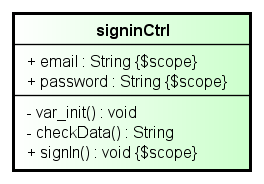
\includegraphics[scale=0.55]{img/diacla/signinCtrl.png}
\caption{Diagramma della classe premi/client/userManager/controllers/signinCtrl}
\end{center}
\end{figure}


\begin{description}
%-------  descrizione della classe%
\item[Descrizione] \hfill
	Controller della view \textit{signin.ng}. Permette all'utente di effettuare il login
	
	
	
%-------  lista delle classi associate%	
\item[Dipendenze] \hfill
	\begin{itemize}
		\item \textbf{premi/client/lib/toastMessageFactory}: per l'invio di notifiche o messaggi di errore all'utente
	\end{itemize}
	
	
%-------  lista degli Attributi%	
\item[Attributi] \hfill
	\begin{description}
		\item[\textbf{+ email : String			}] \hfill
			L'email con cui l'utente si è registrato nel database dell'applicazione
		\item[\textbf{+ password : String			}] \hfill
			La password dell'account dell'utente
	\end{description}
	
	
%-------  lista dei metodi%	
\item[Metodi] \hfill

	% -- inizio metodo -- %
	\begin{description}
		\item[\textbf{\color{blue}- var\_init() : void			}] \hfill
			Inizializza a stringhe vuote email e password
	\end{description}
	% -- fine metodo -- %		
	
	% -- inizio metodo -- %
	\begin{description}
		\item[\textbf{\color{blue}- checkData() : String			}] \hfill
			Controlla che le informazioni scritte dall'utente siano corrette. Restituisce una stringa vuota se corrette, o una descrizione sull'errore rilevato se incorrette
	\end{description}
	% -- fine metodo -- %	
	
	% -- inizio metodo -- %
	\begin{description}
		\item[\textbf{\color{blue}+ signIn() : void			}] \hfill
			Effettua il login sfruttando il metodo loginWithPassword di \$meteor
			Se sono presenti errori invia un messaggio tramite toastMessageFactory, altrimenti manda l'utente alla lista delle presentazioni
	\end{description}
	% -- fine metodo -- %	

\end{description}



%-------  diagramma della classe%
\subsubsection{premi/client/userManager/controllers/signoutCtrl}
\begin{figure}[h]
\begin{center}
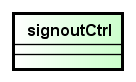
\includegraphics[scale=0.55]{img/diacla/signoutCtrl.png}
\caption{Diagramma della classe premi/client/userManager/controllers/signoutCtrl}
\end{center}
\end{figure}


\begin{description}
%-------  descrizione della classe%
\item[Descrizione] \hfill
	Controller per il logout dell'utente. Chiama la funzione logout di \$meteor e rimanda l'utente alla pagina principale.
	
\end{description}





%-------  diagramma della classe%
\subsubsection{premi/client/userManager/controllers/signupCtrl}
\begin{figure}[h]
\begin{center}
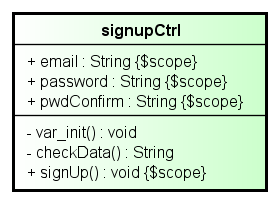
\includegraphics[scale=0.55]{img/diacla/signupCtrl.png}
\caption{Diagramma della classe premi/client/userManager/controllers/signupCtrl}
\end{center}
\end{figure}


\begin{description}
%-------  descrizione della classe%
\item[Descrizione] \hfill
	Controller della view \textit{signup.ng}. Permette all'utente di registrarsi all'interno del database
	
	
	
%-------  lista delle classi associate%	
\item[Dipendenze] \hfill
	\begin{itemize}
		\item \textbf{premi/client/lib/toastMessageFactory}: per l'invio di notifiche o messaggi di errore all'utente
	\end{itemize}
	
	
%-------  lista degli Attributi%	
\item[Attributi] \hfill
	\begin{description}
		\item[\textbf{+ email : String			}] \hfill
			L'email con cui l'utente intende registrarsi
		\item[\textbf{+ password : String			}] \hfill
			La password con cui l'utente intende registrarsi
		\item[\textbf{+ pwdConfirm : String			}] \hfill
			La conferma della password con cui l'utente intende registrarsi
	\end{description}
	
	
%-------  lista dei metodi%	
\item[Metodi] \hfill

	% -- inizio metodo -- %
	\begin{description}
		\item[\textbf{\color{blue}- var\_init() : void			}] \hfill
			Inizializza a stringhe vuote email, password e pwdConfirm
	\end{description}
	% -- fine metodo -- %		
	
	% -- inizio metodo -- %
	\begin{description}
		\item[\textbf{\color{blue}- checkData() : String			}] \hfill
			Controlla che le informazioni scritte dall'utente siano corrette. Restituisce una stringa vuota se corrette, o una descrizione sull'errore rilevato se incorrette
	\end{description}
	% -- fine metodo -- %	
	
	% -- inizio metodo -- %
	\begin{description}
		\item[\textbf{\color{blue}+ signUp() : void			}] \hfill
			Effettua la registrazione sfruttando il metodo createUser di \$meteor
			Se sono presenti errori invia un messaggio tramite toastMessageFactory, altrimenti manda l'utente alla lista delle presentazioni
	\end{description}
	% -- fine metodo -- %	

\end{description}
















